\chapter{Recurrent Neural Networks}
% Authors: Benjamin Ahlbrand (editor), Xingyu Ding, Haoran Anthony Su, 3/12/19.

\section{ High-Level Overview of Recurrent Neural Networks }

As Convolutional Neural Networks naturally lend themselves to images, RNNs (including LSTMs and Transformers) lend themselves similarly to sequential data (which could additionally include each step being images). These might take the form of time series, speech recognition, learning grammars (language translators, name generators, etcetera) or musical rhythms - among others. More precisely one can define them to be directed graphs mapping to a temporal sequence.\\

Visual captioning \cite{DBLP:journals/corr/VinyalsTBE16} is another interesting application, where they combine RNNs and CNNs in order to attempt to generate a text description of a scene \ref{fig:visual_caption}

\begin{figure}
    \centering
    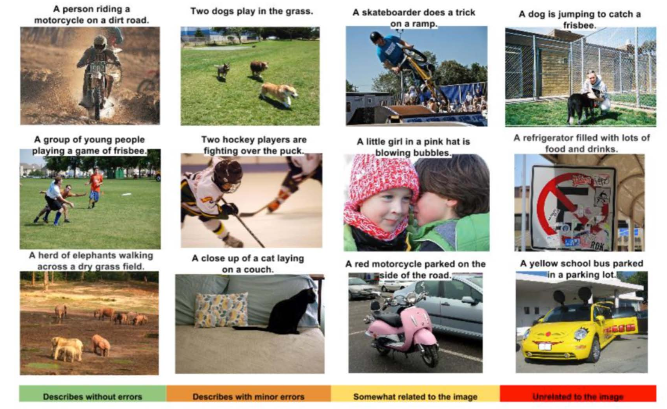
\includegraphics[width=\textwidth]{labs/07/images/image_captioning.png}
    \caption{Vinyals et al. (2016) Show \& Tell: Lessons Learned from the 2015 MSCOCO Image Captioning Challenge}
    \label{fig:visual_caption}
\end{figure}

\subsection{Sequence to vector}
Explanation: input: a sequence of words; output: a scalar value or a vector (see Figure \ref{fig:seq_to_vec}).\\
\begin{figure}[ht]
    \centering
    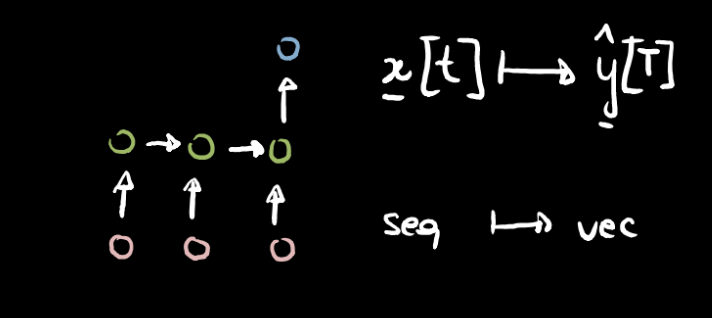
\includegraphics[width=200pt]{labs/07/images/seq_to_vec.png}
    \caption{A hand-drawn diagram showing the sequence to vector rationale in the neural networks. Red, green, blue circles are input,hidden,output nodes, respectively. A sequence of inputs are given to the network and there is only one output in the end.}
    \label{fig:seq_to_vec}
\end{figure}
\\
Example: learning to execute (Zaremba \& Sutskever, 2015)\\
Neural network is trained to interpret several lines of python codes and report the result of the running code (see Figure \ref{fig:learning_to_execute}). \\
\begin{figure}[ht]
    \centering
    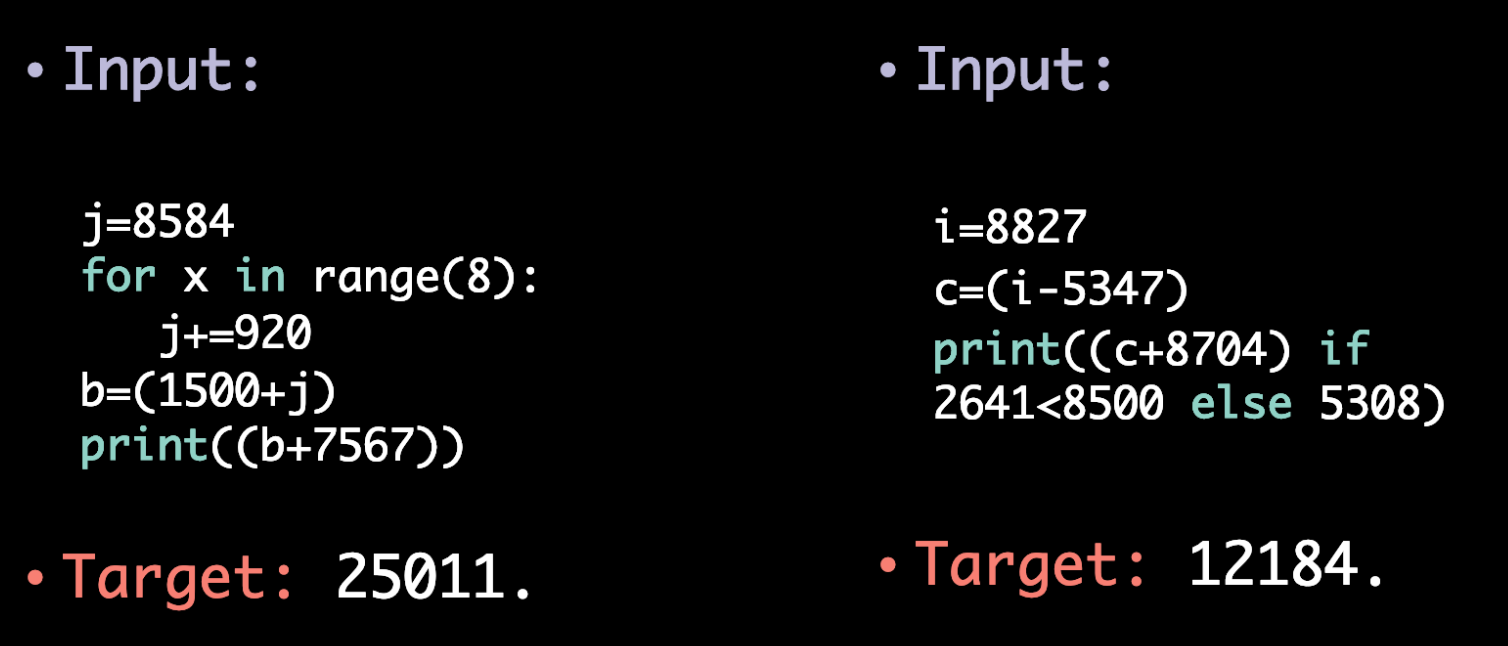
\includegraphics[width=200pt]{labs/07/images/learning_to_execute.png}
    \caption{An example of sequence to vector rationale. A paragraph of Python code is given to the network as an input and the execution output of the Python code is supposed to be the output of the network.}
    \label{fig:learning_to_execute}
\end{figure}

\subsection{Sequence to vector to sequence}
Explanation: a sequence of words $\rightarrow$ hidden representations(vector) $\rightarrow$ output sequence (see Figure \ref{fig:seq_to_vec_to_seq}).\\
\begin{figure}[ht]
    \centering
    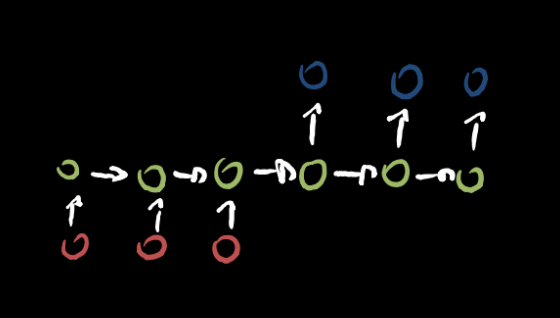
\includegraphics[width=200pt]{labs/07/images/seq_to_vec_to_seq.png}
    \caption{A hand-drawn diagram showing the sequence to vector to sequence rationale in the neural networks. Red, green, blue circles are input,hidden,output nodes, respectively. A sequence of inputs are given to the network and used to compute hidden state. Hidden state variable are  then used to generate a sequence of outputs. }
    \label{fig:seq_to_vec_to_seq}
\end{figure}
\\
Example: phrase representation clustering (Cho et al., 2014)\\
Semantically close phrases are close to each other on the representation map (Figure \ref{fig:phrase_representaion})\\
\begin{figure}[ht]
    \centering
    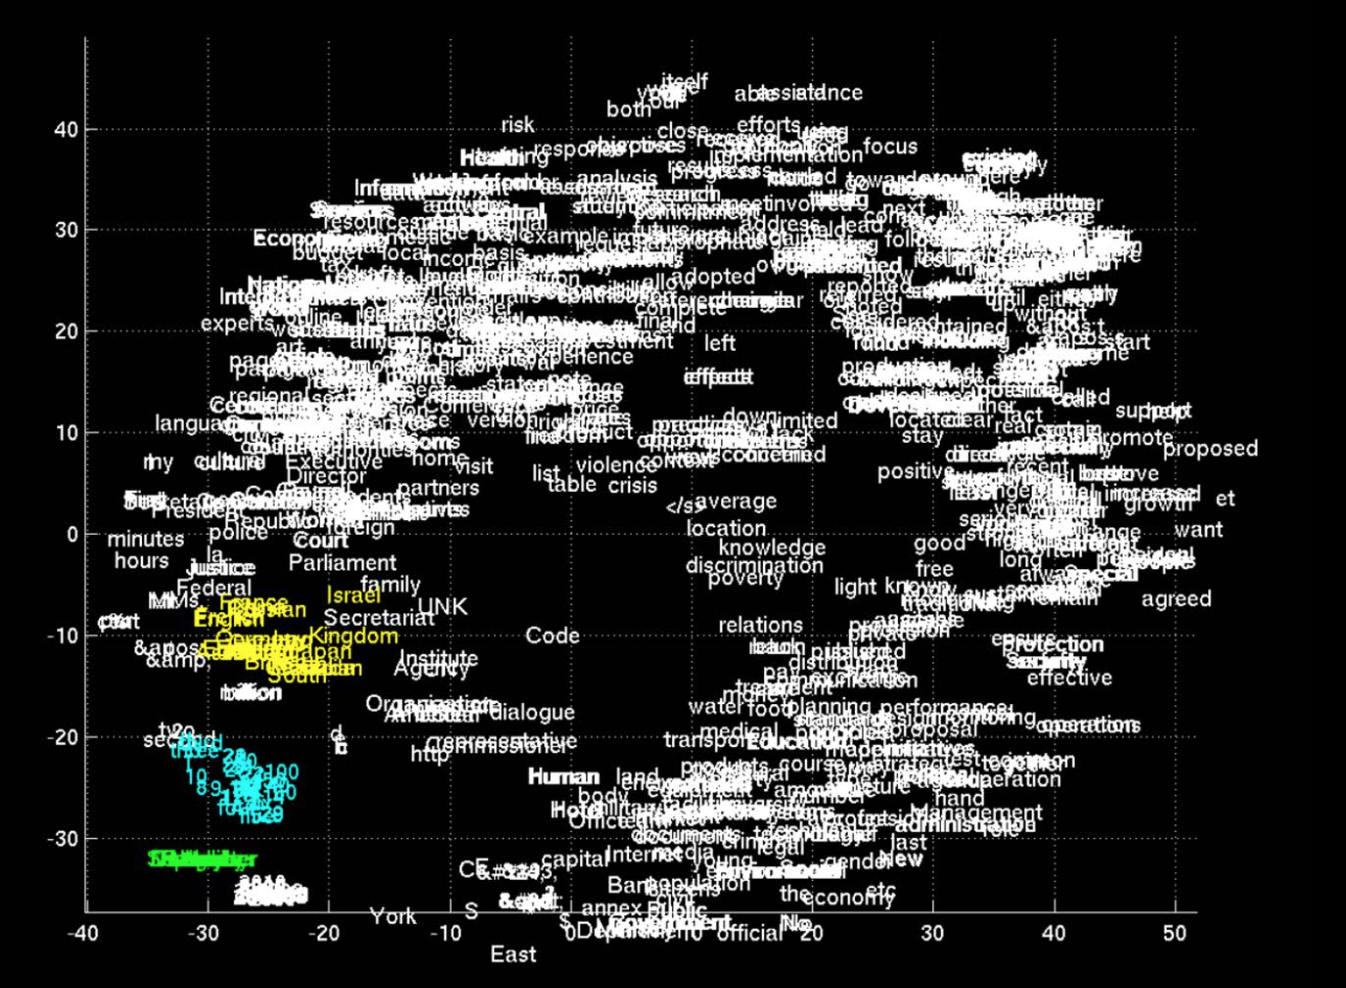
\includegraphics[width=200pt]{labs/07/images/phrase_representation.png}
    \caption{An example of sequence to vector to sequence rationale. Words are clustered according to their semantics}
    \label{fig:phrase_representaion}
\end{figure}
One interesting characteristic is one could perform arithmetic calculation of the semantics in hidden variable space. For example, we have\\
\begin{equation*}
    h('king')-h('men')+h('women')=h('queen')
\end{equation*}
where h(X) is the hidden state of word 'X'. \\

\subsection{Sequence to sequence}
Explanation: a sequence of words $\rightarrow$ another sequence of words (see Figure \ref{fig:seq_to_seq}).\\
\begin{figure}[ht]
    \centering
    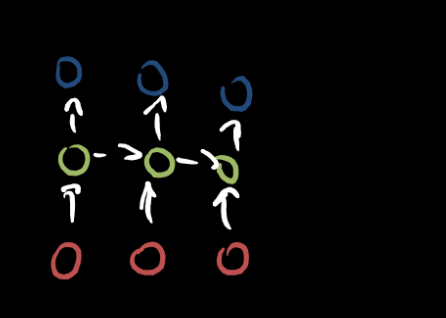
\includegraphics[width=200pt]{labs/07/images/seq_to_seq.png}
    \caption{A hand-drawn diagram showing the sequence to sequence rationale in the neural networks. Red, green, blue circles are input, hidden, output nodes, respectively. A sequence of inputs are given to the network and used to compute hidden state. Hidden state variable are used to generate a sequence of outputs in real time.}
    \label{fig:seq_to_seq}
\end{figure}
\\
Example: auto completion: Once a character is typed, there will be a new sequence of suggestions of auto completion. \\
\\
Example: RNN writer(Sloan(2016))\\
Neural network is trained on sci-fi novels and could be used to auto complete the sci-fi novel.\\
Visit \href{github.com/robinsloan/rnn-writer}{github.com/robinsloan/rnn-writer} for more details.\\

\section{RNN training}
\subsection{BPTT: backpropagation through time}
\begin{figure}[ht]
    \centering
    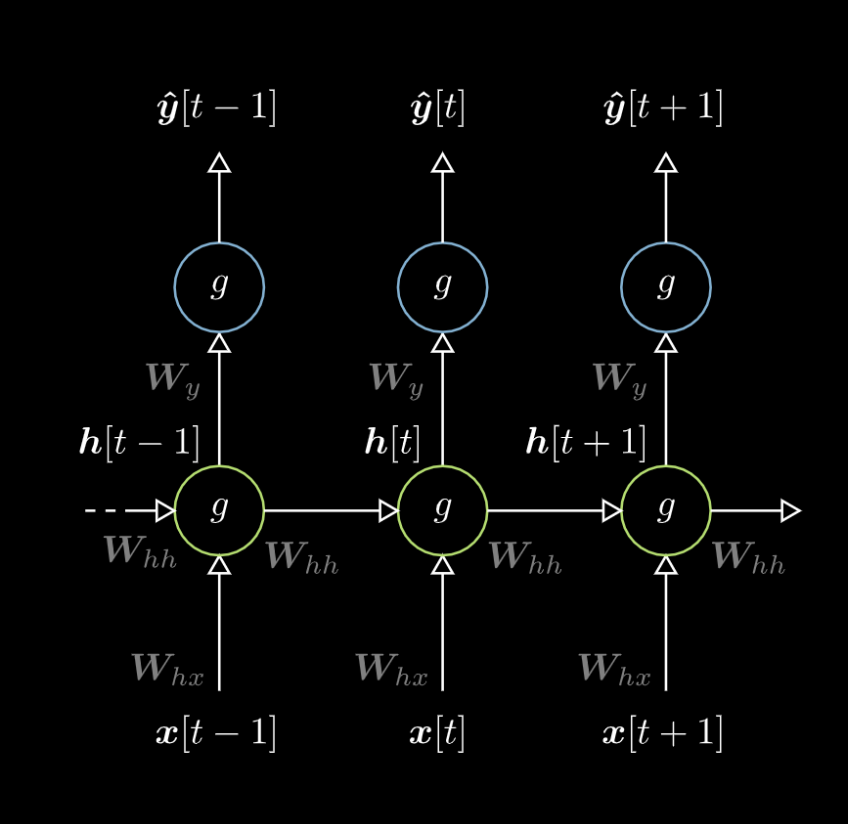
\includegraphics[width=200pt]{labs/07/images/bptt.png}
    \caption{A diagram showing how the values are propagated in a RNN. At each time point t, y is calculated using h from the previous time step and current x.  g() is the transfer function, ReLu for example. h[t] is the value of hidden layer at time t. The initial state of h[t] is 0.}
    \label{fig:bptt}
\end{figure}
In order to train a RNN, we are supposed to use backpropagation through time(BPTT) (see Figure \ref{fig:bptt}). In order to calculate the hidden state value h[t], we have\\
\begin{equation}
h[t] = g(W_{hx}x[t]+W_{hh}h[t-1]+b_h)
\end{equation}
To simplify the equation, we define $W_h$ as
\begin{equation}
    W_h = \begin{bmatrix}W_{hx} & W_{hh}\end{bmatrix}
\end{equation}
Thus, we could rewrite equation 1 as 
\begin{equation}
    h[t] = g(W_h\begin{bmatrix}x[t]\\h[t-1]\end{bmatrix} + b_h)
\end{equation}
$\hat{y}[t]$ could be calculated as shown in figure.\ref{fig:bptt_formula} and then we could use normal backpropagation algorithm except that we sum up the gradients at each time step.  
\begin{figure}[ht]
    \centering
    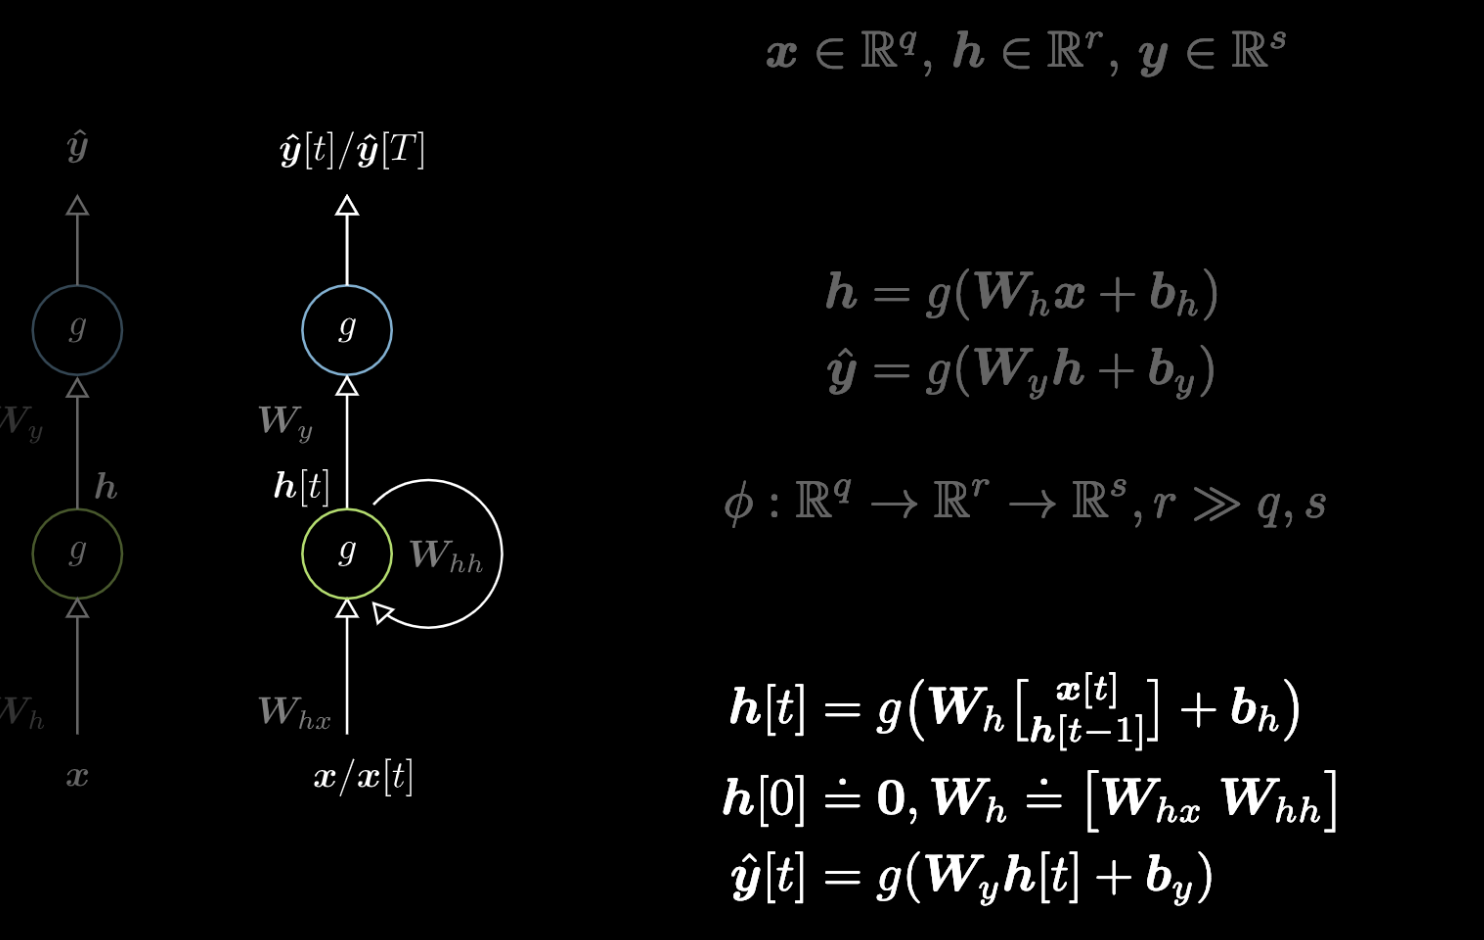
\includegraphics[width=200pt]{labs/07/images/bptt_formula.png}
    \caption{$\hat{y}[t]$ shares the same formula as traditional feedforward network. All we have to do is to use the chain rule and backpropagate the error to previous time step.}
    \label{fig:bptt_formula}
\end{figure}


\section{Batch-ification}
When dealing with text sample with large size, we could slice the text into different batches. For example, the batch-ification process for the following sequence of words should exhibit:\\
\begin{align*}
\begin{bmatrix}
    a & g & m & s\\
    b & h & n & t\\
    c & i & o & u\\
    d & j & p & v\\
    e & k & q & w\\
    f & l & r & x\\
\end{bmatrix}
\end{align*}
In this sequence of words, the batch size is 4. We then determine the input and output for our recurrent neural network, namely:\\
\begin{align*}
X[1:T] & = \begin{bmatrix}
        a & g & m & s\\
        b & h & n & t\\
        c & i & o & u\\
\end{bmatrix}
\end{align*}
\begin{align*}
Y[1:T] & = \begin{bmatrix}
        b & h & n & t\\
        c & i & o & u\\
        d & j & p & v\\
\end{bmatrix}
\end{align*}
Notice here $T = 3$ as we proceed three sequence of words. The next step is to perform back-propagation through time on the sequences of words, which is to say we calculate gradient descent horizontally and vertically. Every time we extract one word from the input sequence and we are aiming to predict the corresponding output in the output sequence. For example, when we select $X[1] = [a, g, m, s]$ as input, we train through the RNN to predict $Y[1] = [b, h, n, t]$. At the same time, we send the hidden representation h[1] forward to perform the RNN given $X[2]$ predicting $Y[2]$. After sending the final hidden representation $h[T-1]$ for the final set of $X[T]$ and $Y[T]$, we cut the gradient and conclude the temporal bulk of this batch. \\

The reason behind concluding the temporal bulk after we sending the last hidden representation of the RNN is that we need to stop the gradient descent eventually. Thus, the gradient descent from the following sequences of words is zero.(The PyTorch Auto-grad will handle this critical point.) Similarly, we also don't have the gradient coming from the past sequences before this batch.

\section{Vanishing of the Gradient and GRU}
The limitation of a recurrent Neural Network is the diminishing of the gradient back in time. A very strong gradient would be weakening back through time because of the way we initialize the weight-by selecting very small eigenvalues across zero. A powerful technique that preventing the gradient from vanishing back through time is by employing Gated Recurrent Unit (GRU).\\

GRU uses two gates-update gates and reset gates. A update gate helps the model to determine how information/gradient from the previous time steps need to pass along to the future. A reset gate, on the other hand, determine how much past information/gradient to forget. 

\section{Long Short Term Memory}
Long Short Term Memory, or typically referred to as LSTMs - these are second order RNNs, tend to imbue a sense of locality (spatial, temporal) to the network models.\\

The forward propagation of the RNN are represented by:\\
\begin{align*}
    h[t] & = g(W_{h} \begin{bmatrix}
        x[t] \\
        h[t - 1] \\
    \end{bmatrix}) + b_{h}\\
    \bar{y}[t] & = g(W_{y}h[t] + b_{y})
\end{align*}
The decomposition of a Gated Recurrent Unit (GRU) will be visualized as:\\
\begin{align*}
i[t] & = \sigma(W_{i} \begin{bmatrix} x[t] \\ h[t - 1] \\ \end{bmatrix}) + b_{i}\\
f[t] & = \sigma(W_{f} \begin{bmatrix} x[t] \\ h[t - 1] \\ \end{bmatrix}) + b_{f}\\ 
o[t] & = \sigma(W_{o} \begin{bmatrix} x[t] \\ h[t - 1] \\ \end{bmatrix}) + b_{o}\\
\bar{c}[t] & = \tanh(W_{c} \begin{bmatrix} x[t] \\ h[t - 1] \\ \end{bmatrix}) + b_{c}\\
c[t] & = f[t] \odot c[t-1] + i[t] \odot \bar{c}[t]\\
h[t] & = o[t] \odot \tanh(c[t])\\
\end{align*}
To control the output, take saturated (squashing / squeezing inputs to a range) sigmoid as an example which we could make the switch simply as 1 or 0, we could determine the hidden representation to be zero by setting the sigmoid function to be null; On the other hand, we could output accordingly by setting the sigmoid function to be 1.\\

To control the memory, we could manipulate the input network and the "don't forget" gate. Simply setting them both to zero, we could reset the memory. To keep the memory, we set the input unit to be zero and memory to be one using the sigmoid function to keep the memory without adding anything from the current input. Finally, we could write to the memory by setting the saturated sigmoid function both to be one to add input to the memory.\\

\section{ Transformers? Pay Attention! }
A new architecture has found popularity in many applications typically dominated by RNNs and LSTMs, Transformers - introduced by \cite{DBLP:journals/corr/VaswaniSPUJGKP17}. Transformers essentially add attention 
RNNs and LSTMs suffer issues with the memory bandwidth bound computations in training, where given the orthogonality of traditional convolutional networks to the GPU hardware, CNNs map perfectly to GPUs. Contrarily these hierachical (sometimes) sequential representations don't typically map quite so easily, and hence, performance suffers as a result.\\